\model{Stack Diagrams}

Each function has its own area of memory to store parameters and other variables.
When a function is invoked, C++ allocates this memory on the \emph{call stack}.
For convenience, we draw ``stack'' diagrams upside down.

\begin{center}
\includegraphics[height=3in]{stack-rings1.png}
\hspace{1em}
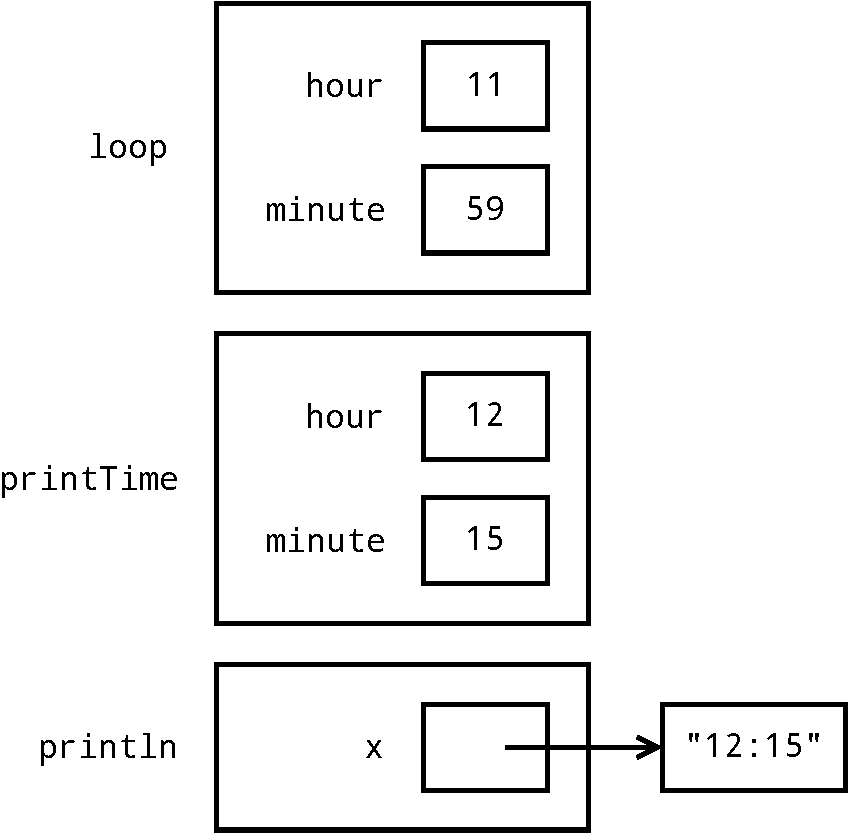
\includegraphics[height=3in]{stack1_loop-crop.pdf}
\end{center}

% \begin{center}
% Note: The signature for \java{System.out.println} is ~\java{public void println(String x)}.
% \end{center}

\begin{javalst}
void printTime(int hour, int minute) {
    Serial.println(String(hour) + ":" + String(minute));
}

void loop() {
    int hour = 11;
    int minute = 59;
    printTime(12, 15);

    while(true) {
    }
}
\end{javalst}



\Q Based on the diagram, how many functions does the program call? \ans{Three}
\vspace{1ex}


\Q Based on the diagram, how many variables does the program have? \ans{Five}
\vspace{1ex}


\Q How is it possible that two variables with the same name can have different values?

\begin{answer}
Each method declares its own variables.
Because they are stored in different memory locations, the values are independent from other methods.
\end{answer}

\newpage

\Q \label{drawing}
Draw a stack diagram to show the state of memory just before \java{println} is called.
Assume the user inputs the value 10.
(You should be able to do this kind of math without a calculator.)

\newpage

